\subsection{Adaptive T-Test}
\frame{\tableofcontents[currentsubsection]}

\begin{frame}{Revisiting the Adaptive T-Test}
\begin{itemize}
    \item Data $X_i \sim \normal\pr{\mu, \sigma^2}$
        with unknown $\mu, \sigma^2$.
    \item $H_0: \mu \leq \mu_0$.
    \item Initial sample size of $n_0$.
    \item $K$ interims where each interim stops 
        if the t-statistic given observed data up to now
        is above the threshold $t^*$.
    \item If continue, add $n_i$ more data.
    \item Final analysis: reject if t-statistic is above $t^*$.
\end{itemize} 
\begin{align*}
    \theta_0 := \frac{\mu}{\sigma^2}
    \quad
    \theta_1 := -\frac{1}{2\sigma^2}
\end{align*}
\end{frame}

\begin{frame}{Tight Analysis Despite Lack of Exact Theory}
\begin{figure}
    \centering
    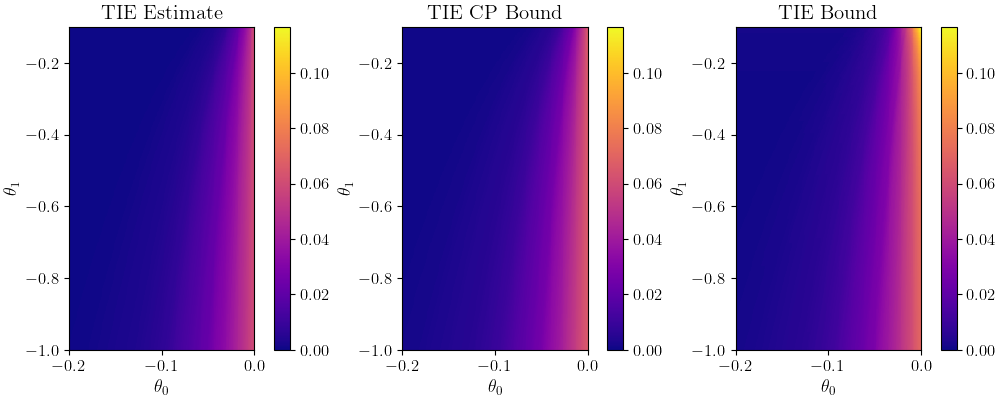
\includegraphics[width=\linewidth]{figs/t_test_adaptive.png}
\end{figure} 
\end{frame}

\begin{frame}{Adaptive T-Test Computation and Configuration}
\begin{itemize}
    \item \textbf{Computation:}
    \begin{itemize}
        \item 327 million simulations.
        \item Runtime: 2s.
        \item M1 Macbook Pro.
    \end{itemize}
    \item \textbf{Configuration:}
    \begin{itemize}
        \item $K=3$ interims.
        \item $n_0 = 100$.
        \item $n_i = 50$ for $1 \leq i \leq K$.
        \item $\mu_0 = 0$.
        \item $\alpha = 0.025$.
    \end{itemize}
\end{itemize}
\end{frame}

\subsection{Bayesian Basket Trial}

\begin{frame}{Bayesian Basket Trial from~\citet{berry:2013}}
\begin{itemize}
    \item Design:
        \begin{align*}
            Y_j &\sim \Binom(n_j, p_j) \quad j=1,\ldots, d \\
            \theta_j &= \theta_{0j} + \logit(p_j) \\
            \theta_j &\sim \normal\pr{\mu, \sigma^2} \\
            \mu &\sim \normal\pr{\mu_0, \sigma_0^2} \\
            \sigma^2 &\sim \Gamma^{-1}\pr{\alpha_0, \beta_0}
        \end{align*}
    \item Let $c \in \br{0,1}^{d-1}$ be a vector of fixed thresholds and $d \equiv 4$.
    \item Reject if $\prob\br{p_i > p_0 | Y} > c_i$ for some null (treatment) arm $i$.
\end{itemize}
\end{frame}

\begin{frame}{Validation shows Type I Error Surface for Bayesian Design}
\begin{figure}
    \centering
    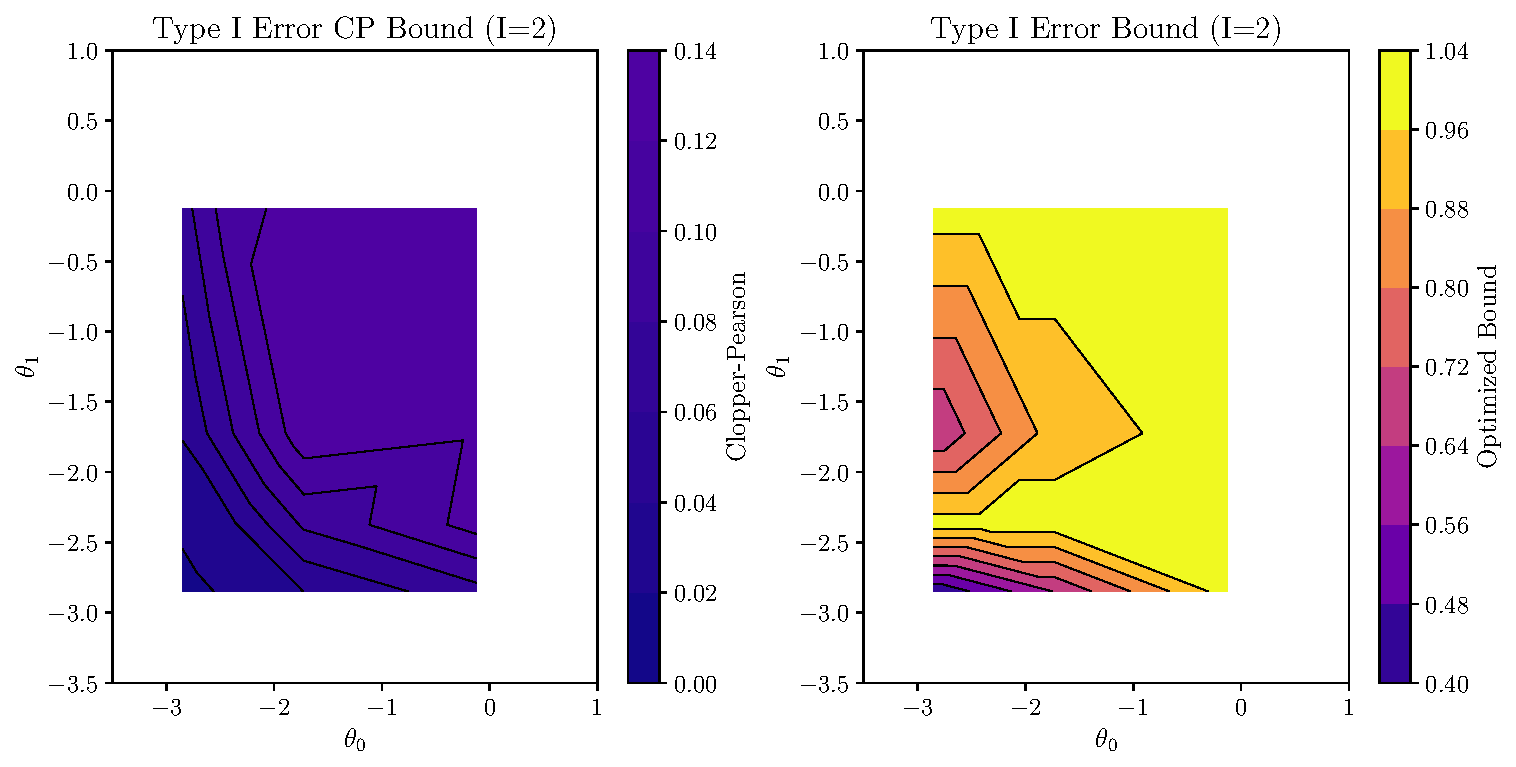
\includegraphics[width=\linewidth]{figs/berry_0.pdf}
\end{figure}
\end{frame}

\begin{frame}{Validation shows Type I Error Surface for Bayesian Design}
\begin{figure}
    \centering
    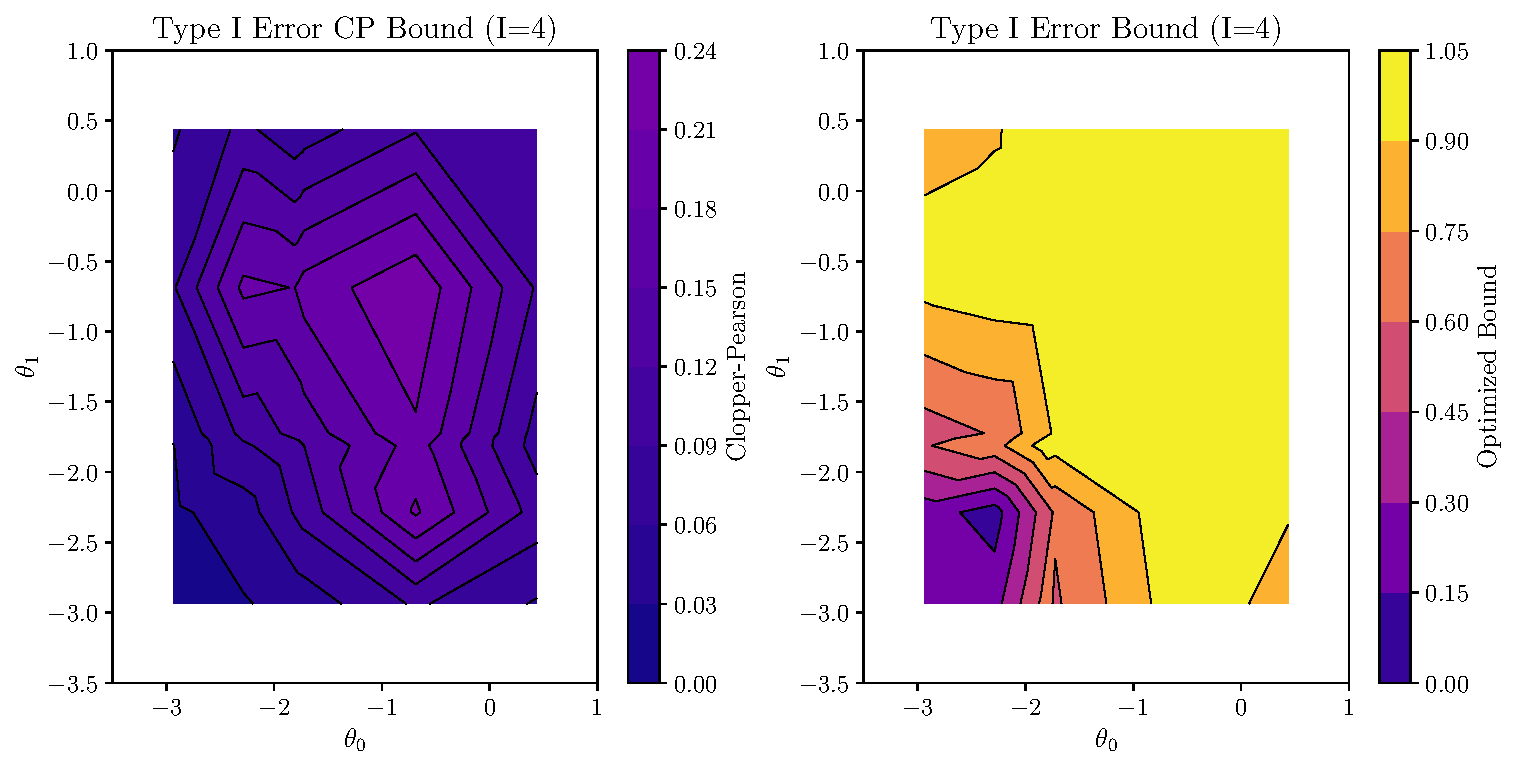
\includegraphics[width=\linewidth]{figs/berry_1.pdf}
\end{figure}
\end{frame}

\begin{frame}{Validation shows Type I Error Surface for Bayesian Design}
\begin{figure}
    \centering
    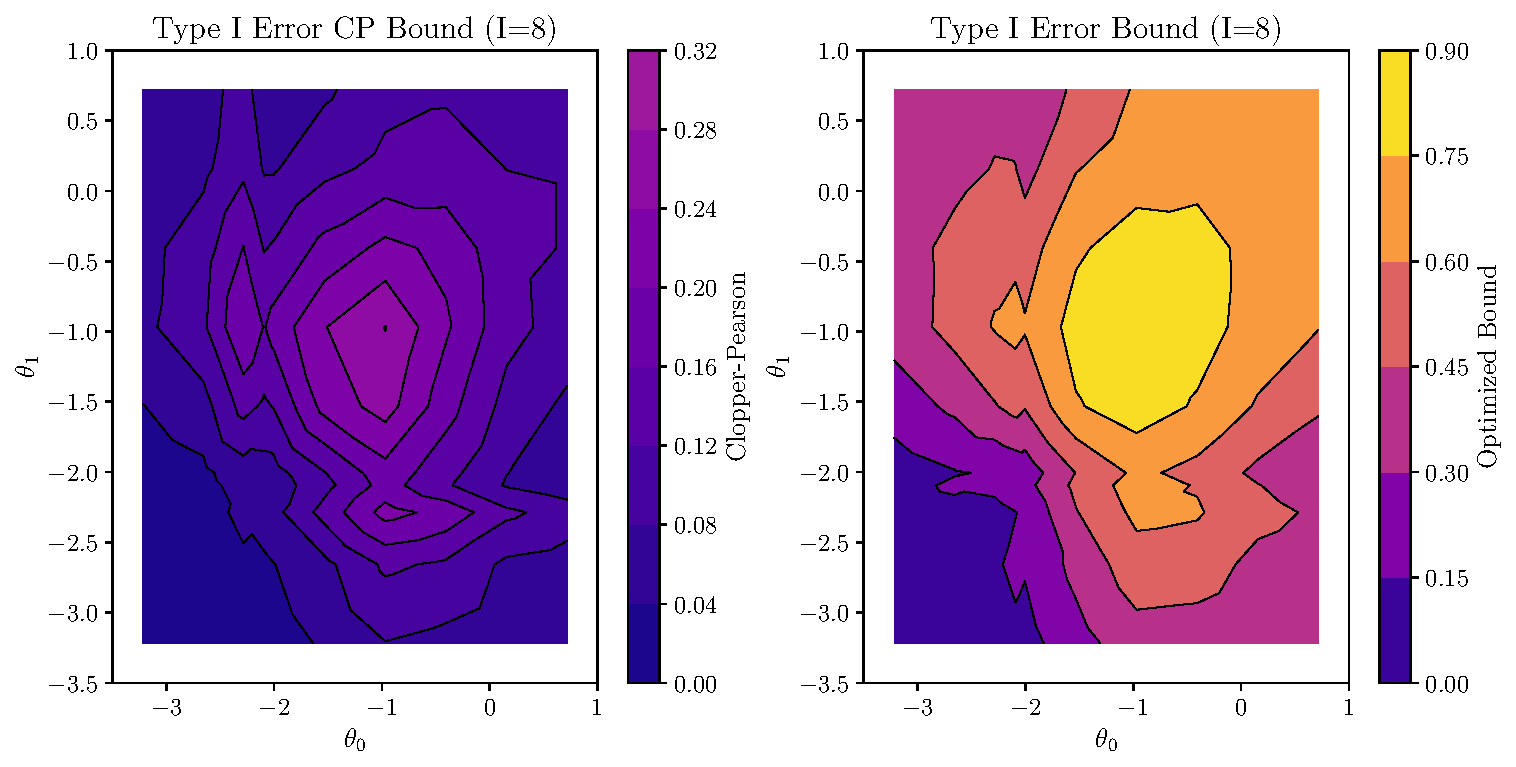
\includegraphics[width=\linewidth]{figs/berry_2.pdf}
\end{figure}
\end{frame}

\begin{frame}{Validation shows Type I Error Surface for Bayesian Design}
\begin{figure}
    \centering
    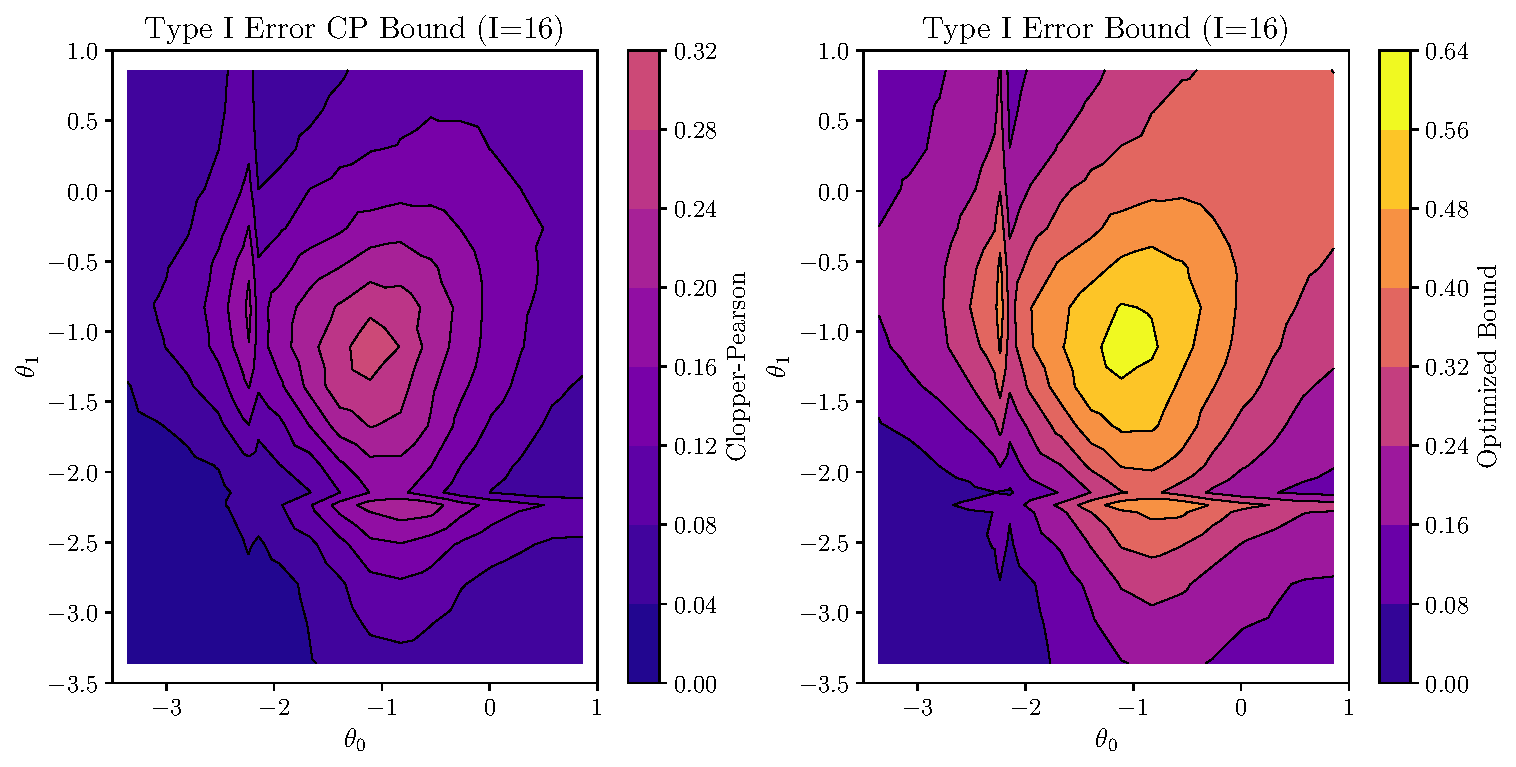
\includegraphics[width=\linewidth]{figs/berry_3.pdf}
\end{figure}
\end{frame}

\begin{frame}{Validation shows Type I Error Surface for Bayesian Design}
\begin{figure}
    \centering
    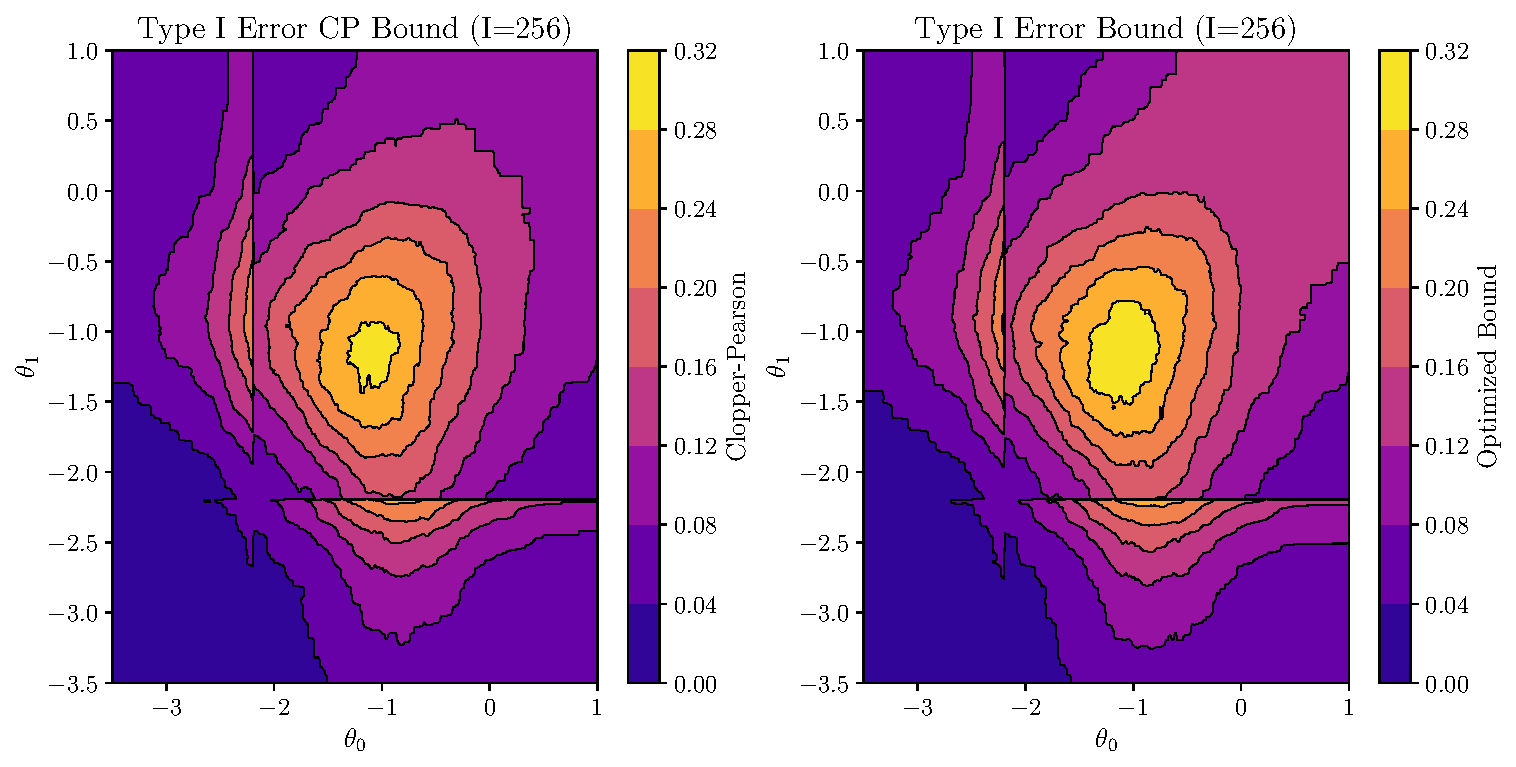
\includegraphics[width=\linewidth]{figs/berry_4.pdf}
\end{figure}
\end{frame}

\begin{frame}{\citet{berry:2013} Computation and Configuration}
\begin{itemize}
    \item \textbf{Computation}:
    \begin{itemize}
        \item 7.34 trillion simulations.
        \item Runtime: 4 hours.
        \item Nvidia V100 GPU.
    \end{itemize}
    \item \textbf{Configuration:}
    \begin{itemize}
        \item $n_i = 35$ for all $i=1,\ldots, d$.
        \item $\mu_0=-1.34$, $\sigma_0 = 10$, $\alpha_0 = 0.0005$, 
            $\beta_0 = 0.000005$.
        \item $c_i = 0.85$ for all $i=1,\ldots, d$.
    \end{itemize}
\end{itemize} 
\end{frame}

%\begin{frame}{\citet{berry:2013} Remarks (Optional)}
%\begin{itemize}
%    \item Type I Error is high in some areas! 
%    \item Type I Error is well-controlled at global null: $\theta_i = \theta_{0i}$.
%    \item This is unsurprising, because ~\citet{berry:2013} had calibrated this design for control only at the global null.
%\end{itemize}
%\end{frame}

\subsection{Complex Phase II/III Selection Design}

\begin{frame}{A Complicated Phase II/III Selection Design}
\begin{itemize}
    \item 3 treatment and 1 control arm with binary outcomes.
    \item Trial decisions using the Bayesian hierarchical model 
        as in~\citet{berry:2013}.
    \item Stage 1: select the ``best'' treatment arm against control
        with interim analyses.
    \item Each of 3 interim analyses can stop for futility,
    drop one or more poorly performing treatments,
    or accelerate an arm to move to stage 2.
    \item Stage 2: one interim and one final analysis. 
    \item The total number of patients across
        all arms and stages is at most 800 with at most 350 in any single arm.
\end{itemize} 
\end{frame}

\begin{frame}{Phase II/III Selection Design Calibrated Successfully}
\begin{figure}
    \centering
    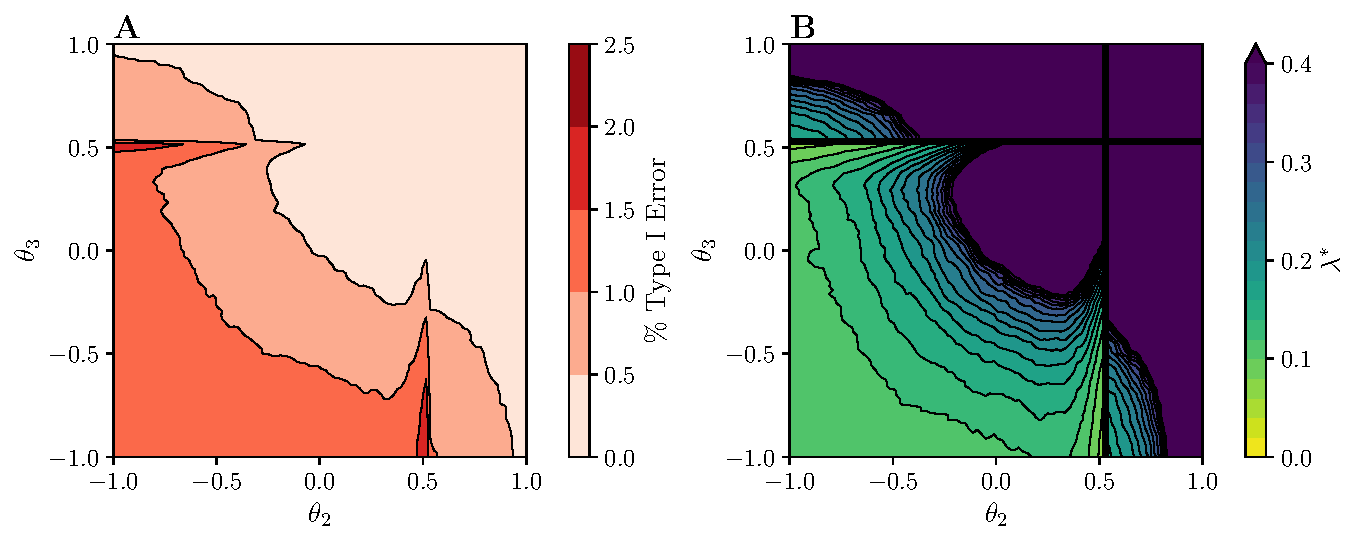
\includegraphics[width=\linewidth]{figs/lewis_tie_lam.pdf}
    \caption{%
    Both plots slice the domain by fixing 2 parameters, $\theta_0 = \theta_1 = 0.533$. Figure \textbf{A} shows the Tilt-Bound profile for the selected threshold $\hat{\lambda}^* = 0.06253$. Figure \textbf{B} shows the critical value $\hat{\lambda}^*_i$ separately for each tile such that its Tilt-Bound is 2.5\%.}
\end{figure} 
\end{frame}

\begin{frame}{Phase II/III Selection Design Computation and Configuration}
\begin{itemize}
    \item \textbf{Computation:}
    \begin{itemize}
        \item 960 billion simulations.
        \item Runtime: 5 days.
        \item Nvidia V100 GPU.
    \end{itemize}
    \item \textbf{Configuration:}
    \begin{itemize}
        \item $H_0: \theta_i \leq \theta_0$ for all $i=1,\ldots, d-1$.
        \item Restrict to $\theta_i \in [-1,1]$ for all $i$.
    \end{itemize}
\end{itemize}
\end{frame}

\begin{frame}{Phase II/III Selection Design Remarks (Optional)}
\begin{itemize}
    \item Max Tilt-Bound occurs at the tile with center
        $\theta_0 = (0.4925, 0.4925, 0.4925, -1.0)$. 
    \item Paradox: worst Type I Error \textbf{does not} 
        occur at the global null (where all treatments perform equally to control), but when \textbf{one} treatment performs poorly.
\end{itemize} 
\end{frame}